
\section{Local Decoders}

\begin{definition}
  Light cone,
\end{definition}

\begin{definition} 
    We say that $D$ is a local decoder if when applied against $2p(1-p)$-depolarized channel: 
    \begin{itemize}
      \item  There exists function $M : (0,1) \rightarrow (0,1) $ such that the probability of each bit being flipped is $M(2p(1-p)) < p^{\frac{100}{99}}$.
      \item There is a constant $l$ such that for any bit, there are only $(\Delta)^{l}$ bits on which the event of it being flipped depends.
    \end{itemize}
For example, if we take $k$ large enough and consider the $(n,k)$-Toric, then both the swift-rule and the flip upon majority are local decoders.
\end{definition}


  \begin{definition}
Consider the moment after the application of the depolarizing channel, and right before the correction by the decoder.

For a subset of qubits $S$, we say that a qubit $x \in S$ is depended if there exists $y \in S$ such:
\begin{enumerate}
  \item Either $x$ and $y$ share a check that is not satisfied. (Type I)  
  \item Or, $x$ and $y$ have checks which share a bit that was flipped by the application of the channel. (Type II)
\end{enumerate}
  \end{definition}


  
  \textbf{Dependence Type I}
  \begin{figure}[h]
    \begin{tikzpicture}[scale=0.7]
      %\draw node at (1.5,4.5) {$v_{2}$ is flipped.};

\draw node (u1) at (3,3) [draw,shape=rectangle]{$u_1$};
\draw node (x) at (0,6) [draw,shape=circle]{$x$};
\draw node (y) at (0,0) [draw,shape=circle]{$y$};
\draw (u1) -- (y)
  (u1) -- (x);
\end{tikzpicture}
  \end{figure}

  \begin{align*}
    & \prb{ (x,y) \in e | u_{1} \text{ is satisfied} }  \\
    & = \prb{ x \in e | u_{1} \text{ is satisfied}  }  \prb{ y \in e | u_{1} \text{ is satisfied}  } \\ 
    & \le \prb{ x \in e }\prb{ y \in e }
  \end{align*}


  \textbf{Dependence Type II}
  \begin{figure}[h]
    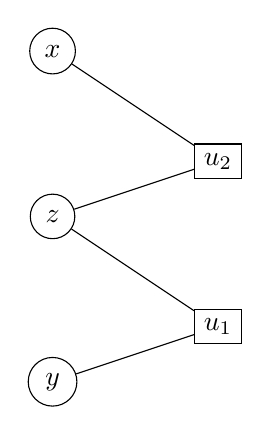
\begin{tikzpicture}[scale=0.7]
      %\draw node at (1.5,4.5) {$v_{2}$ is flipped.};

\draw node (u1) at (3,1) [draw,shape=rectangle]{$u_1$};
\draw node(u2) at (3,4) [draw,shape=rectangle]{$u_2$};
\draw node (x) at (0,6) [draw,shape=circle]{$x$};
\draw node (z) at (0,3) [draw,shape=circle]{$z$};
\draw node (y) at (0,0) [draw,shape=circle]{$y$};
\draw (u1) -- (y)
  (u1) -- (z)
  (u2) -- (x)
  (u2) -- (z);
\end{tikzpicture}
  \end{figure}

  \begin{align*}
    & \prb{ (x,y) \in e | z \text{ is not flipped} }  \\
    & = \prb{ x \in e | z \text{ is not flipped} }  \prb{ y \in e | z \text{ is not flipped} } \\ 
    & \le \prb{ x \in e }\prb{ y \in e }
  \end{align*}


